\lab{Introduction to Bokeh}{Introduction to Bokeh}
\label{lab:Bokeh}

% Written by Tanner Christensen, Summer 2016

\objective{In this lab, we will introduce the Bokeh python package. We will use
Bokeh to produce interactive, dependency-free data visualizations that can
be viewed in any web browser.}

\begin{warn}
This lab uses Bokeh version 0.12.0. It was released in the summer 2016. Bokeh
is still under development, so the syntax is subject to change. However, the
development is far enough along that the general framework has been solidified.
\end{warn}

Bokeh is a visualization package focused on making plots that can be viewed and
shared in web browsers. We have already addressed data visualization practices
in previous labs. In this lab, we will not exhaustively address how to generate
all the plots you have made using matplotlib. Rather, we will highlight some of
the key differences in Bokeh. For all other questions not addressed in this lab,
we direct the reader to the online Bokeh documentation,
\url{http://bokeh.pydata.org/en/0.11.1/}.

\section*{Interactive Visualizations with Bokeh}

One of the major selling points for the Bokeh Python package is the ability to
generate interactive plots that can be viewed a web browser.
The Bokeh Python package is being developed along with a Javascript library
called BokehJS. The Bokeh Python package is simply a wrapper for this library.
The BokehJS library handles all the visualizations in the web browser.

Throughout this lab, all the exercises will piece together to form one final
web-based visualization. To see the final result, go to
\url{THE_FINAL_PROJECT_HOSTED_ON_ACME/data_or_something}.

Even though there are many options for adding interactions to your plots,
(see \url{http://bokeh.pydata.org/en/latest/docs/user_guide/interaction.html})
we will only focus on pan, zoom, hover, and the slider widget.

\section*{Cleaning the Data}
For this project, we will be using the FARS (Fatality Analysis Reporting System)
dataset. This is an incredibly rich data set of all fatal car accidents in the
United States in a given year. We will be examining the data provided from
2010-2014. The data for these years are spread across several files.

\subsection*{The Accidents File}
The columns found in the accidents table contains most of the data we will be
analyzing. For the analysis we will be doing, we will be interested in the
following columns:
\begin{itemize}
    \item ST\_CASE : The unique case ID. This will be used primarily for merging
        information from the other tables.
    \item STATE : State in which the accident occurred. There is a table at the
        end of this lab containing the relationship between IDs and states.
    \item LATITUDE : The latitude of the location where the accident occurred.
        Values of 77.7777, 88.8888, 99.9999 will be considered null.
    \item LONGITUD : The longitude of the location where the accident occurred.
        Values of 777.7777, 888.8888, 999.9999 will be considered null.
        NOTE: Yes, it is spelled ``LONGITUD" without the `E` on the end.

    \item HOUR : Hour of the day when the accident occurred.
    \item DAY : The day of the month when the accidents happened.
    \item MONTH : The month the accident happened.
    \item YEAR : The year the accident happened.
    \item DRUNK\_DR : Number of drunk drivers involved in the accident.
    \item FATALS : The number of fatalities in the accident.
\end{itemize}

\subsection*{The Vehicle File}
The vehicle table is extremely rich. There is an entry for every vehicle involved
in a fatal car accident. Many additional analyses could be performed
on the data here, but we are interested in the following columns:
\begin{itemize}
    \item ST\_CASE : The unique case ID. This will be used primarily for merging
        information from the other tables.
    \item VEH\_NO : The unique vehicle ID identifying each car involved in a given
        accident. This will also be used in merging information from the other
        tables.
    \item SPEEDREL : Whether or not speed was a factor in the car accident. In
        the tables from 2010, 2011, and 2012, the value 0 means No, and the
        value 1 means Yes. In the tables from 2013 and 2014, they begin classifying
        how speed was a factor. The value 0 still means No, and for our purposes,
        values from 2-5 mean Yes. Values of 8 or 9 mean Unknown.
\end{itemize}

\subsection*{The Person File}
The person table is also extremely rich. Each entry contains information for all
persons involved in the accident. For our analyses, we are interested in the
following columns:
\begin{itemize}
    \item ST\_CASE : The unique case ID. This will be used primarily for merging
        information from the other tables.
    \item VEH\_NO : The unique vehicle ID identifying each car involved in a given
        accident. This will also be used in merging information from the other
        tables.
    \item PER\_TYP : The role of this person in the accident. Though the labels in
        this column vary greatly, we will only be interested in entries equal to
        1, signifying the driver.
    \item DRINKING : Whether or not alcohol was involved for this person. The value
        0 means No, 1 means Yes, and 8,9 mean Unknown.
\end{itemize}

The first task is to prepare the DataFrames will we use in our analyses,
the \li{accidents} DataFrame and the \li{drivers} DataFrame.
In the provided file \li{fars_data.zip}, you will find pickle files for accidents,
vehicles, and persons corresponding to each fatal accident. These files are
divided by year, but we want to combine the data from all these years. These
pickle files can be loaded using \li{pd.read_pickle()}.

\begin{problem}
For the \li{accidents} DataFrame, we will need the columns:
\begin{lstlisting}
    ST_CASE, STATE, LATITUDE, LONGITUD, FATALS, HOUR, DAY, MONTH,
    YEAR, DRUNK_DR, SPEEDING.
\end{lstlisting}

The SPEEDING column is derived from
the SPEEDREL column of the vehicles file. The SPEEDREL column describes
which vehicles specifically were speeding. We want the SPEEDING column of this
table to be 0 if no cars were speeding and 1 if any of the cars involved were
speeding. Also, remove all rows containing latitudes or longitudes that we are
considering null due to the criteria described above.

The resulting DataFrame should be 149698 rows x 7 columns. As
another indicator that you have done everything correctly, you should have a total
of 44223 speed related accidents described in the SPEEDING column.

Lastly, the STATE column is all based on IDs. The \li{id_to_state.pickle} file
contains a pickle file with a Python dictionary mapping IDs to states. Replace
all the integer IDs in this column with the corresponding state abbreviation
according to the mapping contained in this dictionary. To load this pickle file,
execute the following code:
\begin{lstlisting}
import pickle
with open("id_to_state.pickle") as file:
    id_to_state = pickle.load(file)
\end{lstlisting}

So in the end your DataFrame should look like this:

\label{my-label}
\begin{tabular}{lllllllllll}
ST\_CASE & STATE & LATITUDE  & LONGITUD   & HOUR & DAY \\
10001    & AL    & 32.641064 & -85.354692 & 4    & 15 \\
10002    & AL    & 31.430447 & -86.956694 & 6    & 11 \\
10003    & AL    & 30.691631 & -88.085778 & 15   & 14 \\
10004    & AL    & 33.868700 & -86.291164 & 1    & 21 \\
10005    & AL    & 33.309742 & -86.787222 & 6    & 4
\end{tabular}

\label{my-label}
\begin{tabular}{lllllllllll}
MONTH & YEAR & DRUNK\_DR & SPEEDING & FATALS \\
1     & 2010 & 1         & 0        & 1      \\
1     & 2010 & 0         & 0        & 1      \\
1     & 2010 & 0         & 1        & 1      \\
1     & 2010 & 0         & 0        & 1      \\
1     & 2010 & 0         & 0        & 1
\end{tabular}

\begin{info}
HINT: Though tedious, it will be easiest to do this whole process correctly if
you do all the needed cleaning for each individual year, then concatenate all
the years together into your final DataFrames. This is due to the fact that
the IDs in the ST\_CASE column are not year specific.
\end{info}
\end{problem}

\begin{problem} \label{prob:convert}
The map we will be using does not does not recognize latitude and longitude
coordinates, but rather coordinates in meters. The FARS data set represents
the location of the accidents in terms of latitude and longitude, so we will
need to convert the coordinate system. This is done with the following code:

\begin{lstlisting}
from_proj = Proj(init="epsg:4326")
to_proj = Proj(init="epsg:3857")

def convert(longitudes, latitudes):
    """Converts latlon coordinates to meters.

    Inputs:
        longitudes (array-like) : array of longitudes
        latitudes (array-like) : array of latitudes

    Example:
        x,y = convert(accidents.LONGITUD, accidents.LATITUDE)
    """

    x_vals = []
    y_vals = []
    for lon, lat in zip(longitudes, latitudes):
        x, y = transform(from_proj, to_proj, lon, lat)
        x_vals.append(x)
        y_vals.append(y)
    return x_vals, y_vals

accidents["x"], accidents["y"] = convert(accidents.LONGITUD, accidents.LATITUDE)
\end{lstlisting}
\end{problem}

\begin{problem}
For the \li{drivers} DataFrame, we will need the columns:
\begin{lstlisting}
    ST_CASE, VEH_NO, PER_TYP, AGE, DRINKING, SPEEDREL, YEAR.
\end{lstlisting}
To obtain the information needed
for this DataFrame, you will need merge the vehicles
file and person file. You will want to merge on ST\_CASE and VEH\_NO.

The resulting DataFrame should be 341436 rows x 7 columns. It is easiest to add
the YEAR column manually. Additionally, we will
only be interested in the entries where PER\_TYP is 1. This brings the final
shape of the DataFrame to 223490 rows x 6 columns (since we can now eliminate
PER\_TYP).

Your DataFrame should look like this:

\begin{tabular}{llllll}
ST\_CASE & VEH\_NO & AGE & DRINKING & SPEEDREL & YEAR \\
10001    & 1       & 51  & 9        & 0        & 2010 \\
10002    & 1       & 44  & 0        & 0        & 2010 \\
10003    & 1       & 27  & 9        & 1        & 2010 \\
10003    & 2       & 45  & 0        & 0        & 2010 \\
10003    & 3       & 28  & 0        & 0        & 2010
\end{tabular}
\end{problem}

Now with the necessary data cleaned, we can dive into the Bokeh package itself.

\section*{Basic Plotting}

The general framework of Bokeh is built on Figures, Glyphs, and Charts.
Figures are analogous to Figure objects in matplotlib. Glyphs consist of any
lines, circles, squares, or patches that we may want to add to the Figure.
Charts are visualizations such as bar charts, histograms, box plots, etc.

There are a few different ways to view your Bokeh plots, but we will address only
two of them. These are \li{output_file()} and \li{output_notebook()}.
If you choose to use \li{output_file}, your Bokeh plot will be saved to an HTML
file that can be viewed in a web browser. This function accepts a string with
the name of the desired filename. If you use \li{output_notebook()}, your Bokeh plots
will appear in your Jupyter Notebook.

\begin{info}
    There may be times that your plots
    may not be behaving as expected. If you are sure there is not a problem with
    your code, try restarting the Bokeh server. Assuming you are working in
    a Jupyter Notebook, this is done by first restarting the kernel, then
    reloading the webpage that hosts your Jupyter Notebook. Additionally, there
    is a currently a memory leak when using \li{output_notebook()}. After
    showing your plot several times in the Jupyter NOtebook, your notebook may
    crash because of losing memory. Again, the solution is restarting the kernel
    and refreshing the webpage.
\end{info}

As has been mentioned already, this lab is not meant to be exhaustive, but
rather is meant to expose you to the basics. For our project, we will be using
Circle glyphs, Square glyphs, Patch glyphs, and Bar charts. Here are some very
basic examples of how to use each of these.

\subsection*{Marker Glyphs (Circles and Squares)}

\begin{comment}
\begin{figure}
\centering
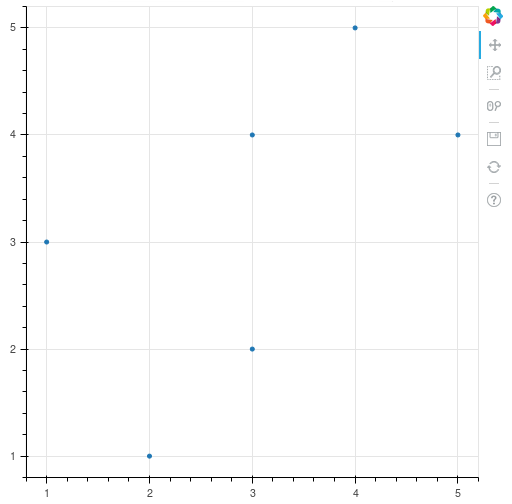
\includegraphics[width=.3\textwidth]{BokehFigs/circles.png} \hfill
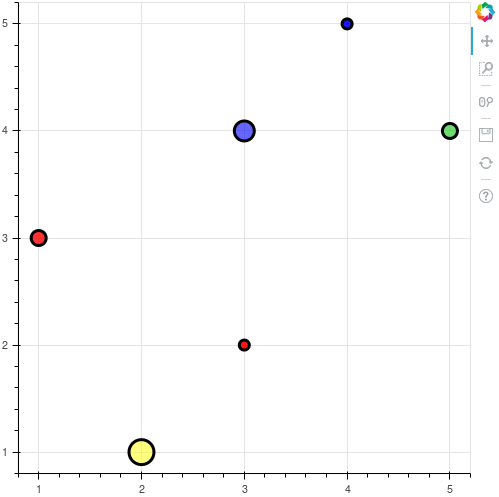
\includegraphics[width=.3\textwidth]{BokehFigs/colored_circles.png} \hfill
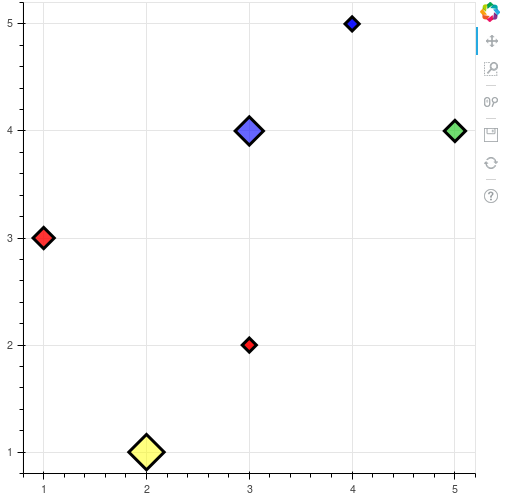
\includegraphics[width=.3\textwidth]{BokehFigs/squares.png}
\end{figure}
\end{comment}


We use Circle glpyhs when we want to plot a collection of circles (such as in
a scatter plot.) The following code example demonstrates the basic syntax of
how this is done.

\begin{lstlisting}
from bokeh.plotting import figure, output_file, show

output_file("my_plot.html")

fig = figure(plot_width=500, plot_height=500)

fig.circle(x=[1,2,3,3,4,5], y=[3,1,2,4,5,4])

show(fig)
\end{lstlisting}

The appearance of marker glyphs is high customizable. There are more than 20 keyword
arguments that allow you to tweak the appearance of your markers. Here are some
of the arguments that are most commonly used.

\begin{itemize}
    \item size : size of marker measured in pixels on screen. So these will
        appear the same size despite the level of zoom.
    \item radius : size of marker measured by radius. These markers will scale
        with the level of zoom.
    \item fill\_color : string of the hex value or the name of the
        color. Valid color names are all colors that have names in HTML.
    \item fill\_alpha : value between 0 and 1 indicating alpha value. 0 indicates
        invisible, 1 indicates opaque.
    \item line\_color : string of the hex value or the name of the
        color of the border. Valid color names are all colors that have
        names in HTML.
    \item line\_alpha : value between 0 and 1 indicating alpha value of the
        border. 0 indicates invisible, 1 indicates opaque.
    \item line\_width : thickness of the border.
\end{itemize}

Additionally, you can pass lists of items to these keyword arguments. The
attributes you specific in these list will be consistent across the indices of
these lists.

\begin{lstlisting}
fig = figure(plot_width=500, plot_height=500)

cir = fig.circle(x=[1,2,3,3,4,5], y=[3,1,2,4,5,4], size=[15,25,10,20,10,15],
            fill_color=["red", "yellow", "red", "blue", "blue", "limegreen"],
            fill_alpha=[.8,.5,.9,.6,.9,.7], line_color="black", line_width=3)

show(fig)
\end{lstlisting}

The syntax for squares is identical. In addition to the keyword arguments listed
above, the \li{angle} keyword argument is also useful for squares.

\begin{lstlisting}
fig = figure(plot_width=500, plot_height=500)

sq = fig.square(x=[1,2,3,3,4,5], y=[3,1,2,4,5,4], size=[15,25,10,20,10,15],
            fill_color=["red", "yellow", "red", "blue", "blue", "limegreen"],
            fill_alpha=[.8,.5,.9,.6,.9,.7], line_color="black", line_width=3,
            angle=np.pi/4)

show(fig)
\end{lstlisting}

\begin{figure}
    \begin{subfigure}{.33\textwidth}
        \centering
            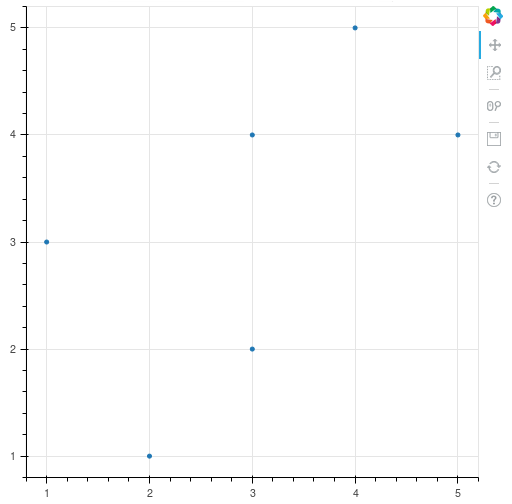
\includegraphics[width=.9\linewidth]{BokehFigs/circles.png}
            \caption{Default circles}
            \label{fig:circles}
    \end{subfigure}%
    \begin{subfigure}{.33\textwidth}
        \centering
            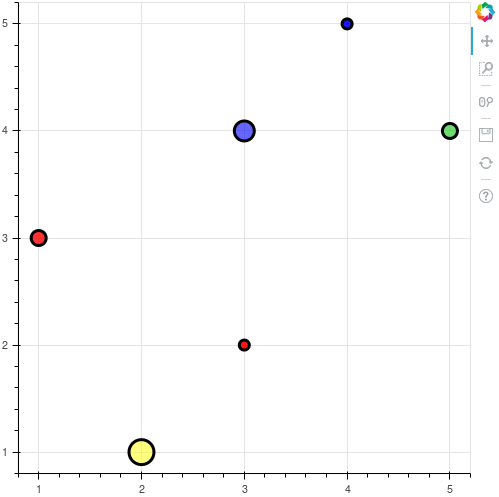
\includegraphics[width=.9\linewidth]{BokehFigs/colored_circles.png}
            \caption{Customized circles}
            \label{fig:circles}
    \end{subfigure}%
    \begin{subfigure}{.33\textwidth}
        \centering
            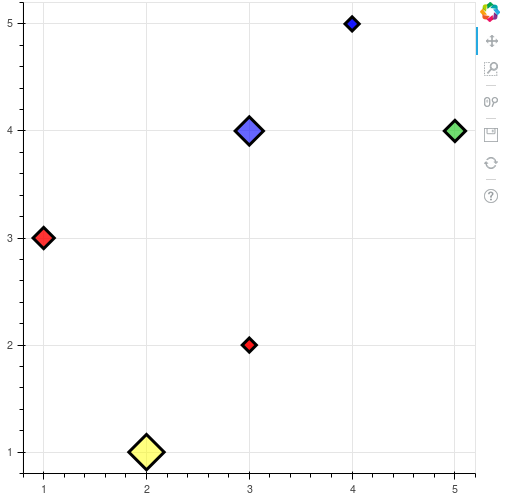
\includegraphics[width=.9\linewidth]{BokehFigs/squares.png}
            \caption{Customized Squares}
            \label{fig:circles}
    \end{subfigure}

\end{figure}

\subsection*{Patch Glyphs}
Patch glyphs are polygon shapes defined by a series of points locating the
corners of the object. These shapes can be very complex. For our project, each
state is a Patch glyph. The syntax for creating Patch glyphs is very similar to
the syntax for creating markers. Most of the keyword arguments are the same as
well.

\begin{lstlisting}
# first iteration of the Sierpinski triangle.
fig = figure(plot_width=500, plot_height=500)

pats = fig.patches(xs=[[1, 3, 2], [3, 5, 4], [2, 4, 3]],
            ys=[[1, 1, 3], [1, 1, 3], [3, 3, 5]],
            fill_color="yellow", line_color="orange",
            line_alpha=.5, line_width=7)

show(fig)
\end{lstlisting}

\begin{figure}
    \centering
        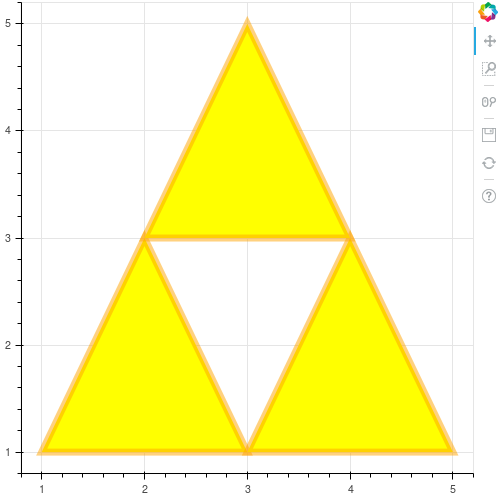
\includegraphics[width=.4\linewidth]{BokehFigs/triforce.png}
        \caption{Collection of patch glyphs}
        \label{fig:circles}
\end{figure}

\subsection*{ColumnDataSource Object}
In the plotting examples we have addressed up to this point, we have expressed
the x and y values explicitly. As mentioned throughout this lab, one of the key
features of Bokeh is to be to interact with your plots. However, if you have
a large dataset, the performance of the interactions can be severely hampered.

Bokeh has a solution for this problem. It comes in the form of the
\li{ColumnDataSource} object. We load our data into this object, connect our
glyph to this object, then if necessary, Bokeh will automatically downsample the
data to maintain acceptable performance. Once a glyph is linked to this source,
you can also change the values in the source to update the positions and attributes
of your glyph. This is an essential component to many of the key features of
Bokeh.

ColumnDataSource objects accept a dictionary or a pandas DataFrame as the source
of data. We reference the different data in this source by the associated key
(in the case of a dictionary) or column name (in the case of a DataFrame).

\begin{lstlisting}
# Replicate the circle marker plot using a DataFrame and ColumnDataSource.
from bokeh.models import ColumnDataSource

fig = figure(plot_width=500, plot_height=500)

df = pd.DataFrame({"x_vals":[1,2,3,3,4,5],
                   "y_vals":[3,1,2,4,5,4],
                   "size":[15,25,10,20,10,15],
                   "fill_color":["red", "yellow", "red", "blue", "blue", "limegreen"],
                   "fill_alpha":[.8,.5,.9,.6,.9,.7]})
cir_source = ColumnDataSource(df)

cir = fig.circle(x="x_vals", y="y_vals", source=cir_source,
            size="size", fill_color="fill_color",
            fill_alpha="fill_alpha", line_color="black", line_width=3)

show(fig)


# Replicate the patches plot using a dictionary and ColumnDataSource.
fig = figure(plot_width=500, plot+height=500)

pat_data = dict("x_vals":[[1, 3, 2], [3, 5, 4], [2, 4, 3]],
                "y_vals":[[1, 1, 3], [1, 1, 3], [3, 3, 5]])

pat_source = ColumnDataSource(data=pat_data)

pats = fig.patches(xs="x_vals", ys="y_vals",
            fill_color="yellow", line_color="orange",
            line_alpha=.5, line_width=7)

show(fig)
\end{lstlisting}

\begin{problem} \label{prob:map}
We will start by adding a map to a Bokeh Figure. Here is the code you will need.
This code will serve as the building block for the rest of this lab.

\begin{lstlisting}
from bokeh.plotting import Figure
from bokeh.models import WMTSTileSource

fig = Figure(plot_width=1100, plot_height=650,
            x_range=(-13000000, -7000000), y_range=(2750000, 6250000),
            tools=["wheel_zoom", "pan"], active_scroll="wheel_zoom")
fig.axis.visible = False

STAMEN_TONER_BACKGROUND = WMTSTileSource(
    url='http://tile.stamen.com/toner-background/{Z}/{X}/{Y}.png',
    attribution=(
        'Map tiles by <a href="http://stamen.com">Stamen Design</a>, '
        'under <a href="http://creativecommons.org/licenses/by/3.0">CC BY 3.0</a>.'
        'Data by <a href="http://openstreetmap.org">OpenStreetMap</a>, '
        'under <a href="http://www.openstreetmap.org/copyright">ODbL</a>'
    )
)

fig.add_tile(STAMEN_TONER_BACKGROUND)
\end{lstlisting}

\end{problem}

\begin{problem} \label{prob:borders}
Using Patch glyphs, draw all the borders for all the
states. The border information you need is found in the pickle file
\li{borders.pickle}. This pickle file contains a nested Python dictionary
where the key is the two letter abbreviation for a given state and the value is
a dictionary containing a list of latitudes and a list of longitudes.

We need a list of lists of x-values and y-values to pass to the
\li{fig.patches()} function. You will need to convert these coordinates the
same way you converted the coordinates in Problem \ref{prob:convert}

To get a list of lists of latitudes and longitudes, you may use the following
code:

\begin{lstlisting}
state_xs = [us_states[code]["lons"] for code in us_states]
state_ys = [us_states[code]["lats"] for code in us_states]
\end{lstlisting}

Draw the state borders using the coordinates defined in \li{state_xs} and
\li{state_ys} and using a \li{ColumnDataSource} object.
\end{problem}

\begin{problem} \label{prob:all_accidents}
Your \li{accidents} DataFrame should contain the converted longitudes and
latitudes for all the fatal accidents.
In the same figure from Problem \ref{prob:borders},
plot a circle for each fatal car accidents. For this problem, you should use
your \li{accidents} DataFrame in conjuction with a ColumnDataSource. For an
added level of detail, color the markers depending on the type of accident:
drunk, speeding, other. The best way to do this would be to have 3 different
\li{ColumnDataSource} objects.
\end{problem}

\subsection*{Speeding up Interactions with WebGL}
As you pan around your figure from Problem \ref{prob:all_accidents}, it may take
a few seconds to load after each movement. This may not be that surprising
considering you have just added approximately 150,000 circles to your figure.
The performence can be improved using WebGL. WebGL stands for Web Graphics
Library. It takes advantage of a compmuter's GPU when plotting a large number of
points.

\begin{problem} \label{prob:webgl}
To take advantage of WebGL, add \li{webgl=True} as a keyword argument to
your figure. You should notice a significant improvement in the response time
while panning and zooming.

\begin{info}
There are times that adding WebGL support to your figure will cause it to behave
strangely. WebGL support is still a fairly new feature of Bokeh. Remember
that Bokeh is still in development, so hopefully things like this will be refined
in time.
\end{info}
\end{problem}

\section*{Adding Tooltips}
It would be useful to display a bit more information on our map. We will
accomplish this with tooltips. When we hover over each state, we will display
a few pieces of key data that may be interesting to the viewer.
To be able to show more information, we will need to prepare a few more
pieces of data.

\begin{problem} \label{prob:lists}
In Problem \ref{prob:borders}, you created two lists of lists, \li{state_xs} and
\li{state_ys}. When hovering over a Patch glyph, Bokeh keeps track which index
corresponds with that Patch. For our tooltips, we will need a few more lists. We
have to take extra special care that the indices of all these lists are
consistent.

Using list comprehension again, create a list of state abbreviations, a list of
the total number of accidents by state, a list of the percentage of speed-related
accidents by state, and a list of the percentage of drunk driving accidents by
state.

There is more than one correct way to do this, but whatever method you choose to
use, take extra care to make sure that the indices correspond to the same state
across all these lists.
\end{problem}

\begin{figure}
    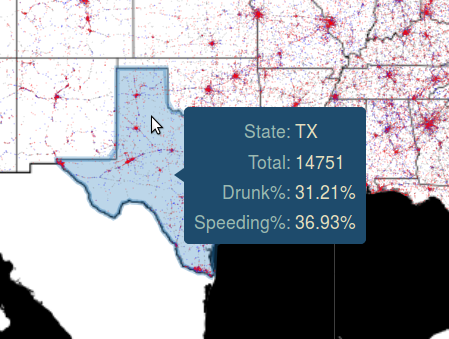
\includegraphics[width=.5\linewidth]{BokehFigs/hover.png}
    \caption{Example of state hover tooltip.}
    \label{fig:hover}
\end{figure}

\subsection*{HoverTool and Tooltips}
Adding tooltips to Patch glyphs is fairly straightforward. The process is best
explained by first presenting an example.

\begin{lstlisting}
import numpy as np
from bokeh.plotting import figure, output_notebook, show
from bokeh.models import HoverTool, ColumnDataSource

x_vals = [[0,1,0], [0,1,1], [1,2,1], [1,2,2]]
y_vals = [[0,0,1], [1,1,0], [0,0,1], [1,1,0]]

x_coords = [0,0,1,1,2,2]
y_coords = [0,1,0,1,0,1]

fig = figure(plot_width=500, plot_height=300)
col = ["Blue", "Red", "Yellow", "Green"]

patch_source = ColumnDataSource(
    data=dict(
        col=col,
        x_vals=x_vals,
        y_vals=y_vals
    )
)

circle_source = ColumnDataSource(
    data=dict(
        x_coords=x_coords,
        y_coords=y_coords
    )
)

triangles = fig.patches("x_vals", "y_vals", color="col", source=patch_source,
           line_color='black', line_width=3, fill_alpha=.5, line_alpha=0
           hover_color="col", hover_alpha=.8, hover_line_color='black')
circles = fig.circle("x_coords", "y_coords", fill_color='black', source=circle_source,
           fill_alpha=.5, hover_color="black", hover_alpha=1, line_alpha=0, size=18)

fig.add_tools(HoverTool(renderers=[triangles], tooltips=[("Color", " @col")]))
fig.add_tools(HoverTool(renderers=[circles], tooltips=[("Point", " (@x_coords, @y_coords)")]))

show(fig)
\end{lstlisting}

Now let's piece apart this example. Notice first that we have a
\li{ColumnDataSource} object for the patch coordinates and another
\li{ColumnDataSource} for the circles. In general, it is a good idea to separate
\li{ColumnDataSource} objects like this, but more specifically, we need to do this
because we want to have two different hover behaviors.

Next, notice that there are some keyword arguments included in these glyphs we
have not discussed yet. The keyword arguments \li{hover_color}, \li{hover_alpha},
and \li{hover_line_color}. When hovering over one of these glpyhs, these arguments
overwrite \li{fill_color}, \li{fill_alpha}, and \li{line_color}, respectivley.

Finally, when creating the \li{HoverTool} object, you will most commonly use
the \li{renderers} and \li{tooltips} keyword arguments. The \li{renderers}
argument accepts a list of glyphs. At times, there is unpredicted behavior if you
include more than one glpyh in this list. The \li{tooltips} arguments functions
just like the \li{tooltips} argument we discussed in the section on bar charts.

\begin{problem} \label{prob:hover_map}
On your plot of the United States, we can provide much more information to this
plot using tooltips. Using the lists you prepared in Problem \ref{prob:lists},
add tooltips for the Patch objects in this plot. Also adjust the appearence of
the Patch objects under the mouse so it is clear which state is being selected.

Your tooltips should look similar to Figure \ref{fig:hover}.

\end{problem}



\section*{Adding More Complicated Interactions Using Widgets}
\begin{info}
At the beginning of this lab, we mentioned that Bokeh is still in development
so some explanations will need to be updated. There is some material in this
section that is still under active development. In theory, the code presented
here will still work, but it is quite possible that there will be a better way
to do these tasks in the future.
\end{info}

One of the mottos the Bokeh developers have is, \emph{We write the Javascript so
you don't have to.} If you happen to have experience with Javascript, you can
do some pretty amazing things with Bokeh interactions. In this section, we
address some of the interactions that are possible without using Javascript.

\subsection*{Select}
The Select widget is ideal for changing attributes of the figure where you want
to allow only a few different options. The code for creating Select widgets is
very straightforward.

\begin{lstlisting}
from bokeh.io import output_file, show
from bokeh.models.widgets import Select

output_file("select.html")

select = Select(title="Option:", value="one",
                options=["one", "two", "three", "four"])

show(select)
\end{lstlisting}

For our project, we want to be able to
give the user the ability to gain information from the first map without needing
to hover over each individual state. Since we are interested in drunk driving
accidents and speeding accidents, it makes sense to give the user the option to
color the states according to the percentage of these types of accidents.

To be able to accomplish this, we will need to have some way of knowing if the
value in the Select widget has changed, and if it has, what we should do with the
new value.

Most Bokeh widgets have a \li{on_change} method. This method is called whenever
a certain parameter (usually \li{"value"}) is changed. Here is a simple example.

\begin{lstlisting}
import pandas as pd
import numpy as np
from bokeh.io import curdoc
from bokeh.plotting import Figure
from bokeh.models import ColumnDataSource, Select
from bokeh.layouts import column

COUNT = 10
df = pd.DataFrame({"x":np.random.rand(COUNT),
                   "y":np.random.rand(COUNT),
                   "color":"white"})
source = ColumnDataSource(df)

fig = Figure()
fig.circle(source=source, x="x", y="y", fill_color="color",
           line_color="black", size=40)

select = Select(title="Option:", value="white",
                options=["white", "red", "blue", "yellow"])

def update_color(attrname, old, new):
    source.data["color"] = [select.value]*COUNT

select.on_change('value', update_color)

curdoc().add_root(column(fig, select))
\end{lstlisting}

There are a few things to point out with this example. Note that we have a function
called \li{update_color}. This function is called whenever the \li{"value"} of
the Select widget is changed. The function arguments \li{attrname, old, new}
are used by Bokeh, but you don't need to worry about them at all in this lab.
Because we have our Circle glyph tied to a
\li{ColumnDataSource}, any change to this source will affect the Circle glpyh.

Second, note that we have not specified an \li{output_file}. Instead, we use
\li{curdoc()}, which stands for ``current document". We add the layouts we want
to the current document through the \li{add_root()} method. In our case, we
stack all the elements of our document using the \li{column()} function. You can
learn more about possible layouts here:
\url{http://bokeh.pydata.org/en/latest/docs/user_guide/layout.html}

Using the \li{on_change} function requires a Bokeh Server to be running.
You can view the code above by executing
\begin{lstlisting}
$ bokeh serve <FILENAME>.py
\end{lstlisting}
in your terminal, then going to \li{localhost:5006/<FILENAME>} in your web
browser.

\begin{problem}
In this problem, we will add a Select widget to our map. This Select widget will
specify the color map we wish to use for the states.

In your Select widget, have options for \li{"None"}, \li{"Drunk \%"}, and
\li{"Speeding \%"}. To assign the states the appropriate color, you may use
the following code, or you may adjust the functionality as you like.

\begin{lstlisting}
# change this first line if you want a different colormap
from bokeh.palettes import Reds9

COLORS.reverse()
no_colors = ['#FFFFFF']*len(state_names)
drunk_colors = [COLORS[i] for i in pd.qcut(state_percent_dr, len(COLORS)).codes]
speeding_colors = [COLORS[i] for i in pd.qcut(state_percent_sp, len(COLORS)).codes]
\end{lstlisting}

This code assumes you have lists named \li{state_names}, \li{state_percent_dr},
and \li{state_percent_sp} from Problem \ref{prob:lists}.

Changing the values of the select box should result in something similar to
Figure \ref{fig:select}.
\end{problem}

\begin{figure}
    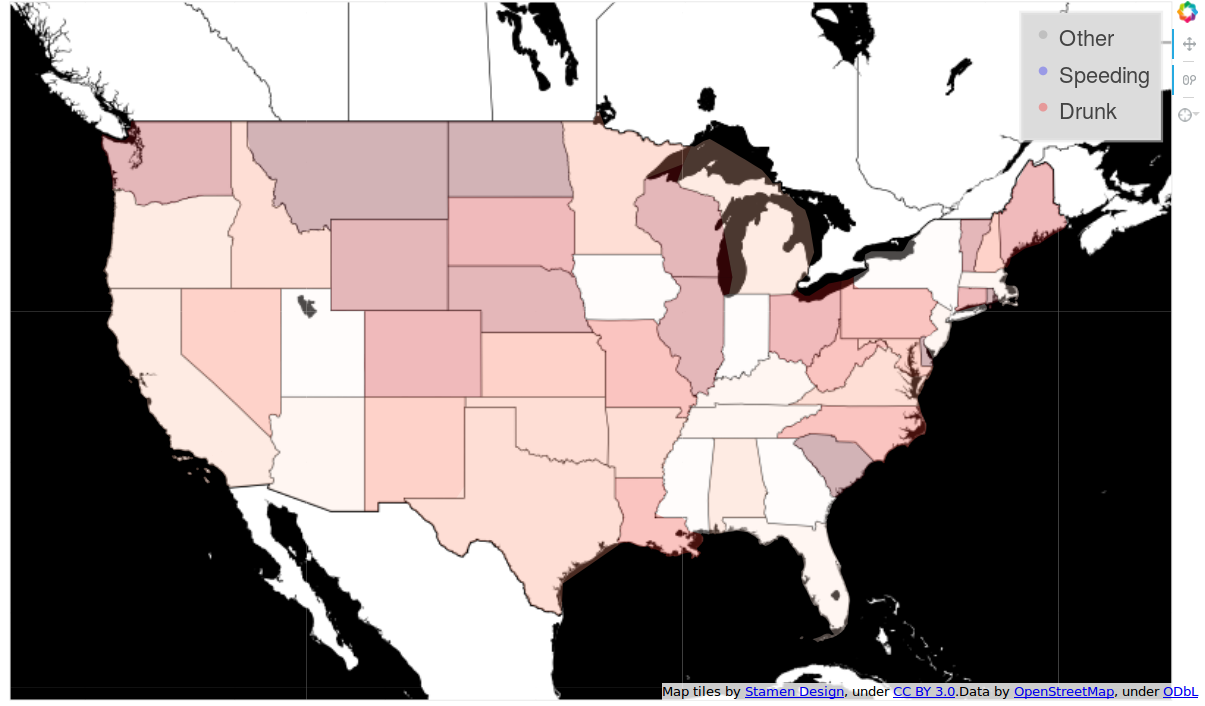
\includegraphics[width=.7\linewidth]{BokehFigs/color_states.png}
    \caption{Example of coloring states based on percentage of drunk
            driving fatalities.}
    \label{fig:select}
\end{figure}

%====SUPPLEMENTAL MATERIALS====

\begin{comment}

\subsection*{Interactions in Jupyter Notebook}

\section*{Tying It All Together}

\subsection*{Tab}

\section*{Suggestions for Further Learning}

\begin{itemize}
    \item Streaming data
    \item Dashboards
    \item Data Exploration (crossfilter)
\end{itemize}



\section*{Supplemental Stuffs}

\section*{Basic Charts}
Like in pandas, it is very easy to make visualizations in Bokeh from DataFrames.
Bokeh provides very accessible tools for creating bar charts, histograms, box
plots, and scatter plots.

\begin{problem} \label{prob:counts}
Before making the bar charts for this project, we will need to clean the data a
little bit more. In your \li{drivers} DataFrame, we are interested in the columns
AGE, DRINKING, and SPEEDREL. For the bar charts, creating an additional DataFrame
will greatly simplify this task. Create a DataFrame called \li{counts} that has
columns,
\begin{itemize}
    \item AGE : age of drivers
    \item SPEEDING : number of drivers that where speeding when the accident
                occurred.
    \item NOT\_SP : number of drivers that were NOT speeding when the accident
                occurred.
    \item UN\_SP : number of drivers that were involved in accidents where the
                role of speed was unknown.
    \item DRUNK : number of drivers that were driving drunk when the accident
                occurred.
    \item NOT\_DR : number of drivers that were NOT driving drunk when the
                accident occurred.
    \item UN\_DR : number of drivers that were involved in accidents where the
                role of drinking was unknown.
\end{itemize}
\end{problem}

\subsection*{Bar Charts}
Now with the \li{counts} DataFrame ready, we will focus on creating a stacked
bar chart using this data.

To initialize a Bokeh Bar Chart, we pass a pandas DataFrame and indicate what
the label (x-axis) and values (y-axis) for the chart will be. The following
code will create a bar chart that displays the number of drunk driving accidents
based on age.

\begin{lstlisting}
from bokeh.charts import Bar

b = Bar(counts, label="AGE", values="DRUNK")

show(b)
\end{lstlisting}

When creating a stacked bar chart, we use an operation called \li{blend}. This
groups columns of your DataFrame together in preparation for stacking the
columns. The following code creates a stacked bar chart that displays the number
of drivers in speed-related accidents by age.

\begin{lstlisting}
from bokeh.charts.operations import blend
speed_bar = Bar(counts,
              values=blend("UN_SP", "SPEEDING", "NOT_SP",
                          name="totals", labels_name="speed"),
              label="AGE",
              stack="speed")
show(speed_bar)
\end{lstlisting}

\begin{problem}
Following the example above, create a stacked bar chart that displays the
number of drivers in drunk-driving-related accidents by age.
\end{problem}

\section*{Adding Tooltips to Visualizations}
Tooltips allow the user to gain more insight from the visualization.
The process of tooltips differs depending on the type of visualization.
We will address how to add hover interactions to bar charts and patch glyphs.

\subsection*{Adding Tooltips to Bar Charts}
With the stacked bar charts made in the last section, it is difficult to
distinguish the age and exact number of people represented by each bar.
Tooltips will be  particularly useful for clarifying these pieces of the data.

Luckily, adding tooltips to bar charts is very easy. In fact, it is just a matter
of adding a keyword argument. Here is a refined version of the code displaying
drunk-driving-related accidents by age.

\begin{lstlisting}
b = Bar(counts, label="AGE", values="DR",
        tooltips=[("AGE","@AGE"), ("TOTAL", "@height")])
show(b)
\end{lstlisting}

The \li{tooltips} keyword argument is a list of tuples. The first entry in the
tuple is the key and the second entry is the value. The value \li{"@AGE"}
references what the which column is being selected. The value \li{"@height"} is
a builtin option that displays the height of the selected bar.

\begin{problem}
Add a tooltip to both of the stacked bar charts. Include at least the age and
total number of people per category.
\end{problem}

\subsection*{Slider}
Sliders are very useful when slicing across sections of data or adjusting
attributes of glyphs. If adjusting attributes of a glyph, it makes more sense to
use a Slider rather than a Select widget if you have a range of valid values.

\begin{lstlisting}
import pandas as pd
import numpy as np
from bokeh.io import curdoc
from bokeh.plotting import Figure
from bokeh.models import ColumnDataSource, Slider
from bokeh.layouts import column

COUNT = 10
df = pd.DataFrame({"x":np.random.rand(COUNT), "y":np.random.rand(COUNT), "radius":0.05})
source = ColumnDataSource(df)

fig = Figure()
fig.circle(source=source, x="x", y="y", fill_color="red", line_color="black", radius="radius")

slider = Slider(start=1, end=10, step=0.1, value=5)

def update_size(attrname, old, new):
    source.data["radius"] = [slider.value / 100.]*COUNT

slider.on_change('value', update_size)

curdoc().add_root(column(fig,slider))
\end{lstlisting}

\begin{problem}
In this problem, you will create a figure that allows the user to interact with
the data in multiple ways. Create a Slider widget that displays the accidents by
hour. Also include a HoverTool for the accident markers that displays a tooltip
with the format:
\begin{itemize}
    \item Date: MM/DD/YEAR
    \item Fatalities: NUMBER OF FATALITIES
    \item Drunk: YES/NO
    \item Speeding: YES/NO
\end{itemize}

\end{problem}

\end{comment}
